\documentclass[usenames,dvipsnames]{beamer}
\usepackage[utf8]{inputenc}
\usepackage[english]{babel}
\usepackage{graphicx}
\usepackage{tikz}
\usepackage{amsmath}
\usepackage{amsthm}
\usepackage{amssymb}
\usepackage{mathtools}
\usepackage{csquotes}
\usepackage{tabularx,pbox}
% tikz packages
\usetikzlibrary{positioning}
\usepackage{physics}
\usepackage{yhmath}
\usepackage{cancel}
\usepackage{color}
\usepackage{siunitx}
\usepackage{array}
\usepackage{multirow}
\usepackage{gensymb}
\usepackage{tabularx}
\usepackage{extarrows}
\usepackage{booktabs}
\usetikzlibrary{fadings}
\usetikzlibrary{patterns}
\usetikzlibrary{shadows.blur}
\usetikzlibrary{shapes}


\definecolor{carminepink}{rgb}{0.92, 0.3, 0.26}
\definecolor{candypink}{rgb}{0.89, 0.44, 0.48}

% theme
\usetheme[numbering=counter, progressbar=foot, titleformat=allcaps]{metropolis}  
\setbeamercolor{title separator}{fg=BrickRed}
\setbeamercolor{progress bar in head/foot}{fg=BrickRed}
\setbeamercolor{alerted text}{fg=BrickRed}

\newcommand{\tabitem}{~~\llap{\textbullet}~~}

\title{Markov Chain Analysis of \\The Ehrenfest Urn Model}
\date{2020/2021}
\author{Elena Acinapura}
\institute{Università di Trento}

\begin{document}
  \maketitle

  \begin{frame}{Contents}
    \MakeUppercase{\textbf{The Ehrenfest urn model}}

    \bigskip
    \MakeUppercase{\textbf{Analysis via Markov chains}}
      \begin{itemize}
        \item Limiting distribution
        \item Mean recurrence time
      \end{itemize}
      \bigskip
    \MakeUppercase{\textbf{Simulation}}
  \end{frame}

  \section{Motivation}
  \begin{frame}{Irreversibility vs Recurrence}
    \begin{center}
      Thermodynamic processes such as
    \end{center}
    \begin{table}
        \begin{center}
        \begin{tabular}{l c}
            \tabitem diffusions & \\
            \tabitem heat transfers & $\rightarrow \quad $ \alert{\MakeUppercase{irreversible}}\\
            \tabitem phase transitions & 
        \end{tabular}
        \end{center}
    \end{table}
    
    \begin{center}
        \textbf{but}
    \end{center}
    
    \begin{center}
    Newtonian mechanics $\quad \rightarrow \quad$ \alert{\MakeUppercase{time-reversible}}
    \end{center}
  \end{frame}

  \begin{frame}[standout]
    \textsc{A statistical approach}
  \end{frame}
  

  \section{The Ehrenfest Urn Model}
  \input{model}

  
  \section{Markov chain analysis}
  \begin{frame}{Markov chains - definitions}
    \begin{center}
      \Large{\textbf{Discrete Markov chains}}
    \end{center}
    A mathematical theory for stochastic processes

    The state of the system $X$ is a random variable

    \bigskip
    \begin{figure}
      


\tikzset{every picture/.style={line width=0.75pt}} %set default line width to 0.75pt        

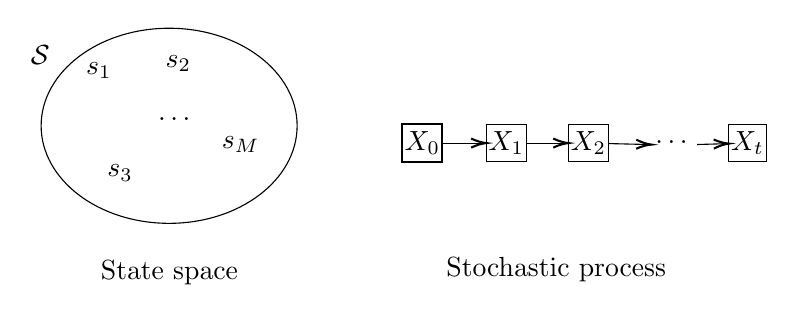
\begin{tikzpicture}[x=0.50pt,y=0.50pt,yscale=-1,xscale=1]
%uncomment if require: \path (0,928); %set diagram left start at 0, and has height of 928

%Shape: Ellipse [id:dp18659796531361872] 
\draw   (59.33,412.31) .. controls (59.33,373.38) and (100.75,341.81) .. (151.83,341.81) .. controls (202.92,341.81) and (244.33,373.38) .. (244.33,412.31) .. controls (244.33,451.25) and (202.92,482.81) .. (151.83,482.81) .. controls (100.75,482.81) and (59.33,451.25) .. (59.33,412.31) -- cycle ;

% Text Node
\draw (50,352.15) node [anchor=north west][inner sep=0.75pt]    {$\mathcal{S}$};
% Text Node
\draw (100.67,507.81) node [anchor=north west][inner sep=0.75pt]   [align=left] {State space};
% Text Node
\draw (90,364.48) node [anchor=north west][inner sep=0.75pt]    {$s_{1}$};
% Text Node
\draw (147.33,359.81) node [anchor=north west][inner sep=0.75pt]    {$s_{2}$};
% Text Node
\draw (105.33,438.81) node [anchor=north west][inner sep=0.75pt]    {$s_{3}$};
% Text Node
\draw (142,404.15) node [anchor=north west][inner sep=0.75pt]    {$\dotsc $};
% Text Node
\draw (188,418.15) node [anchor=north west][inner sep=0.75pt]    {$s_{M}$};
% Text Node
\draw  [line width=0.75]   (320.36,411.31) -- (349.36,411.31) -- (349.36,438.31) -- (320.36,438.31) -- cycle  ;
\draw (334.86,424.81) node    {$X_{0}$};
% Text Node
\draw    (381.03,411.31) -- (410.03,411.31) -- (410.03,438.31) -- (381.03,438.31) -- cycle  ;
\draw (395.53,424.81) node    {$X_{1}$};
% Text Node
\draw    (440.36,411.31) -- (469.36,411.31) -- (469.36,438.31) -- (440.36,438.31) -- cycle  ;
\draw (454.86,424.81) node    {$X_{2}$};
% Text Node
\draw    (556.37,411.31) -- (583.37,411.31) -- (583.37,438.31) -- (556.37,438.31) -- cycle  ;
\draw (569.87,424.81) node    {$X_{t}$};
% Text Node
\draw (501.33,420.81) node [anchor=north west][inner sep=0.75pt]    {$\dots $};
% Text Node
\draw (350.33,505.81) node [anchor=north west][inner sep=0.75pt]   [align=left] {Stochastic process};
% Connection
\draw    (349.36,424.81) -- (379.03,424.81) ;
\draw [shift={(381.03,424.81)}, rotate = 180] [color={rgb, 255:red, 0; green, 0; blue, 0 }  ][line width=0.75]    (10.93,-3.29) .. controls (6.95,-1.4) and (3.31,-0.3) .. (0,0) .. controls (3.31,0.3) and (6.95,1.4) .. (10.93,3.29)   ;
% Connection
\draw    (410.03,424.81) -- (438.36,424.81) ;
\draw [shift={(440.36,424.81)}, rotate = 180] [color={rgb, 255:red, 0; green, 0; blue, 0 }  ][line width=0.75]    (10.93,-3.29) .. controls (6.95,-1.4) and (3.31,-0.3) .. (0,0) .. controls (3.31,0.3) and (6.95,1.4) .. (10.93,3.29)   ;
% Connection
\draw    (469.36,425.16) -- (498.33,425.86) ;
\draw [shift={(500.33,425.91)}, rotate = 181.39] [color={rgb, 255:red, 0; green, 0; blue, 0 }  ][line width=0.75]    (10.93,-3.29) .. controls (6.95,-1.4) and (3.31,-0.3) .. (0,0) .. controls (3.31,0.3) and (6.95,1.4) .. (10.93,3.29)   ;
% Connection
\draw    (533.33,425.85) -- (554.37,425.25) ;
\draw [shift={(556.37,425.19)}, rotate = 538.38] [color={rgb, 255:red, 0; green, 0; blue, 0 }  ][line width=0.75]    (10.93,-3.29) .. controls (6.95,-1.4) and (3.31,-0.3) .. (0,0) .. controls (3.31,0.3) and (6.95,1.4) .. (10.93,3.29)   ;

\end{tikzpicture}
    \end{figure}
  \end{frame}

  \begin{frame}{Markov chains - definitions}
    \begin{center}
      \Large{\textbf{Markov property}}
    \end{center}
    \begin{table}
      \begin{tabularx}{\textwidth}{c >{\raggedright}X}
        \alert{\emph{Memorylessness}}: & only the current state influences the next transition \tabularnewline
      \end{tabularx}
    \end{table}
  \end{frame}

  \begin{frame}{Markov chains --- definitions}
    \begin{center}
      \Large \textbf{Representing probabilities}
    \end{center}

    \renewcommand{\tabularxcolumn}{m}
    \begin{table}
      \begin{tabularx}{0.9\textwidth}{c c >{\raggedright}X}
        \alert{Distribution} & $\rightarrow$ & probabilities for the system to be in the various possible states \tabularnewline
        & & \tabularnewline
        \alert{Stochastic matrix} & $\rightarrow$ & probabilities of the possible transitions
      \end{tabularx}

    \end{table}
    
  \end{frame}

  \begin{frame}{Markov chains and the Ehrenfest model}
    \Large In the Ehrenfest model:
    \normalsize
    \begin{itemize}
      \item<1-> state $X = $ number of particles in box A
      \item<2-> possible values: $0, \dots, N$
      \item<3-> example
    \end{itemize}
    
    \begin{figure}[r]
      \only<3>{\input{pictures/example_state}}
    \end{figure}
  \end{frame}

  \begin{frame}[standout]
    \textsc{A sequence of states of the Ehrenfest model is a Markov chain}\\
    \vspace{30pt}
    \textsc{The \enquote{Ehrenfest chain}}
  \end{frame}


  \section{Asymptotic behaviour}
  \begin{frame}{LIMITING DISTRIBUTION}
    \centering
    Evolution for $t$ time steps\\\medskip
    $\downarrow$\\\medskip
    Does the distribution converge as $t \rightarrow \infty$?\\\medskip
    $\downarrow$\\\medskip
    \alert{Limiting distribution}\\\medskip
    $\downarrow$\\\medskip
    Concept of \alert{equilibrium}
  \end{frame}

  \begin{frame}{STATIONARY DISTRIBUTION}
    \centering
    \Large \textbf{Stationary distribution}
    \normalsize
    \begin{itemize}
      \item distribution that \alert{remains the same} after one timestep
      \item \alert{eigenvector} of the stochastic matrix with unitary eigenvalue
    \end{itemize}
  \end{frame}

  \begin{frame}[standout]
    \textsc{The limiting distribution is a stationary distribution}
  \end{frame}

  \begin{frame}
    \Large
    \centering
    \dots\ \textsc{however, a stationary distribution is not always the limiting distribution}
    
    \vspace{40pt}

    \normalsize
    The \alert{Perron-Frobenius theorem} gives the sufficient conditions
  \end{frame}

  \begin{frame}{Asymptotic limit of the Ehrenfest chain}
    \Large 
    \centering
    \vspace{30pt}
    Limiting distribution of the Ehrenfest chain\\
    \vspace{20pt}
    \MakeUppercase{\alert{Binomial distribution}}\\
  \end{frame}
  
  \begin{frame}{Asymptotic limit of the Ehrenfest chain}
    \vspace{30pt}
    Example with $N = 10$
    \begin{figure}
      \includegraphics[scale = 0.5]{pictures/binomial.pdf}
    \end{figure}
  \end{frame}

\end{document}